%================================================================
\chapter{Results and Discussion}\label{chap:results_discussion}
%================================================================
In this chapter, we will detail how various models presented in previous chapters were configured and trained. The models will also be characterized using aforementioned numerical methods, and the results will be compared to earlier research.

The vanishing gradient phenomenon will be investigated for QNNs, QCNs and DNNs by studying the magnitude of their gradients (see \autoref{sec:BackwardPropagationQCN} and \autoref{sec:BackpropogationDNN}). This will be done for different architectures, especially different number of layers.

We will characterize the geometry of the loss landscape of QCNs(see \autoref{sec:Quantum Circuit Network}) and other models by studying the EFIM presented in \autoref{sec:EFIM}. The result will be used to asses the trainability of different models and predict how architecture affects training.

To assess the expressivity of QCNs and compare them to other models, we will use trajectory length as presented in \autoref{sec:TrajectoryLength}. This will be done for both trained and untrained models.

In order to test models in a practical setting, and give support to previous results and analyses in this thesis, the models will be trained to fit gaussian data. This will be done both using idealised simulation(see \autoref{sec:Exact Expectation Value}), and simulated, noisy hardware(see).


%================================================================
\section{Vanishing Gradient Phenomenon}\label{sec:Vanishing Gradient Phenomenon}
%================================================================
We start by investigating the magnitude of the gradient for QNNs for different number of qubits and repetitions of the ansatz. To construct the QNNs, we use qubit encoding with $R_x$ rotations together with the simple ansatz. To derive an output, we estimate the parity of the state exactly using the methods outlined in see \autoref{sec:Exact Expectation Value} and \autoref{sec:Inference}. 
Instead of investigating the gradient of some loss function, i.e. \autoref{eq:LossDerivateWRTparameter}, we will investigate the gradient of the model output itself, $\frac{\partial f(\boldsymbol{x^{(i)}};\boldsymbol{\theta})}{\partial \theta_j}$. If this quantity vanishes, it follows that also \autoref{eq:LossDerivateWRTparameter} also vanishes, for any loss function and labels $y$.

To get a result representative of a realistic feature space, we will sample features uniformly from $\boldsymbol{x}^{(i)} \sim U(-\frac{\pi}{2}, \frac{\pi}{2})$, as explained in (ost). The QNNs will also be initialized in the standard way, i.e. sampling parameters as $\theta_j \sim U(-\frac{\pi}{2}, \frac{\pi}{2})$. The resulting magnitude of the gradients for different number of qubits and ansatz repetitions can be seen in figure 

\begin{figure}[htp]
    \centering
    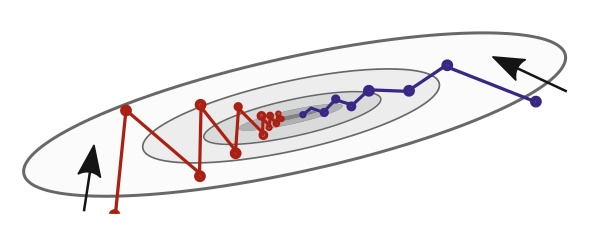
\includegraphics[width=8cm]{latex/figures/thin_vally.png}
    \caption{Two-dimensional representation of the loss landscape for a parameterized model, illustrating a thin valley. The optimization steps in red showcase optimization without momentum. Optimization steps in blue implement momentum, showing dampened oscillation and better convergence. The figure is retrieved from \citet{SupervisedwquantumComputers}.}
    \label{fig:thinValley}
\end{figure}


%================================================================
\section{Investigating the Loss Landscape}\label{sec:Investigating the Loss Landscape}
%================================================================
We explore the geometry of the loss landscape of various models by studying the eigenvalue spectrum of the EFIM. Looking \autoref{eq:EmpiricalFisher}, we see that the EFIM, unlike the Hessian, is independent of targets $y^{(i)}$. This makes the analysis problem independent, and characterises only the models and their architectures. The input data $\mathcal{X} = \{\boldsymbol{x}^{(1)}, \cdots, \boldsymbol{x}^{(N)}\}$, used for calculating the EFIM, is sampled randomly from a standard normal distribution as $\mathcal{X} \sim N(0,1)^{(N,p)}$. This ensures that the input is evenly sampled from feature space and is consistent with the analysis of \citet{abbas2020power}.  Here, we use $N=200$ samples and either $p=4$ or $p=6$ inputs, depending on the model. For each unique model, the EFIM is calculated 10 times for different random initializations of the parameters(see stuff). The resulting spectrum is then averaged over the 10 initializations to produce more significant results. For a complete description of the models analysed in this section, see \autoref{tab:FIM models}.

\begin{table}[H]
\centering
\begin{tabular}{|l|l|l|l|l|l|l|l|}
\hline
Model &Type & Qubits& Reps & Layers & Width & Encoder        & $n_{\theta}$ \\ \hline
A    & QNN & 4& 18   & 1      & 4     & RZZ Encoding   & 72  \\ \hline
B    & QCN & 4& 3    & 2      & 4     & Qubit Encoding & 60 \\ \hline
C    & QCN & 4& 2    & 3      & 4     & Qubit Encoding & 72  \\ \hline
D    & QCN & 4& 1    & 5      & 4     & Qubit Encoding & 68  \\ \hline
E    & DNN & NA& NA   & 3      & 6     & NA             & 79 \\ \hline
F    & QNN & 6& 26   & 1      & 6     & RZZ Encoding   & 156  \\ \hline
G    & QCN & 6& 4    & 2      & 6     & Qubit Encoding & 168 \\ \hline
H    & QCN & 6& 2    & 3      & 6     & Qubit Encoding & 156  \\ \hline
I    & QCN & 6& 1    & 5      & 6     & Qubit Encoding & 150  \\ \hline
J    & DNN & NA& NA   & 3      & 9     & NA             & 163 \\ \hline
\end{tabular}
\caption{Description of the architecture of the models analysed in this section. The QNN and QCN models use exact evaluation of parity to derive outputs (see \autoref{sec:Exact Expectation Value} and \autoref{sec:Inference}). The DNN models uses sigmoid activation in all layers. The parameters of the models are appropriately initialized as presented in (stuff).} 
\label{tab:FIM models}
\end{table}

\autoref{fig:FIM Comparison} compares the EFIM spectrum of QNNs, QCNs and DNNs. Their architectures are chosen so that the models have approximately equal number of parameters. This is to ensure a fair comparison. Looking at the spectra of the DNN models, we see the characteristic result of a singular large eigenvalue, with the rest sitting close to zero. This indicates that DNN models exhibit a loss landscape that is very flat in all but one direction, where it is extremely distorted. This result is consistent with the findings of \citet{abbas2020power} and \citet{karakida2019universal}. As explained in \autoref{sec:Optimization}, this geometry of the loss landscape is often associated with slower optimization. Further, we see that the spectra of the our QNN models are much more uniformly distributed compared to the DNN models. This results in a loss landscape that is significantly distorted in most directions, rather than just one. \citet{abbas2020power} came to the same conclusion for their QNN models, and argued that this uniformity of the spectrum meant that landscape was more well-condition for optimization. They strengthened this hypothesis by showing numerically that QNNs trained faster than DNNs. 

\begin{figure}[H]
    \centering
    \begin{subfigure}[t]{0.5\textwidth}
        \centering
        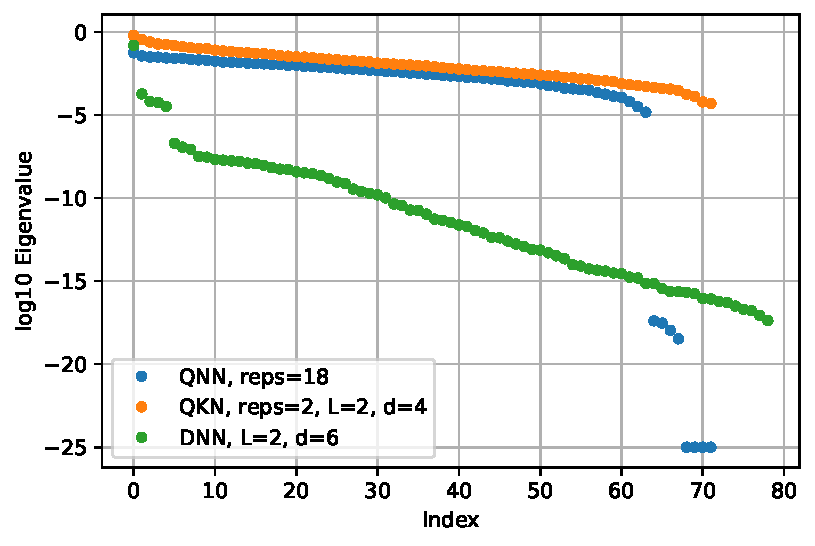
\includegraphics[height=1.9in]{latex/figures/FIM_qubits_4.pdf}
        \caption{Lorem ipsum}
        
    \end{subfigure}%
    ~ 
    \begin{subfigure}[t]{0.5\textwidth}
        \centering
        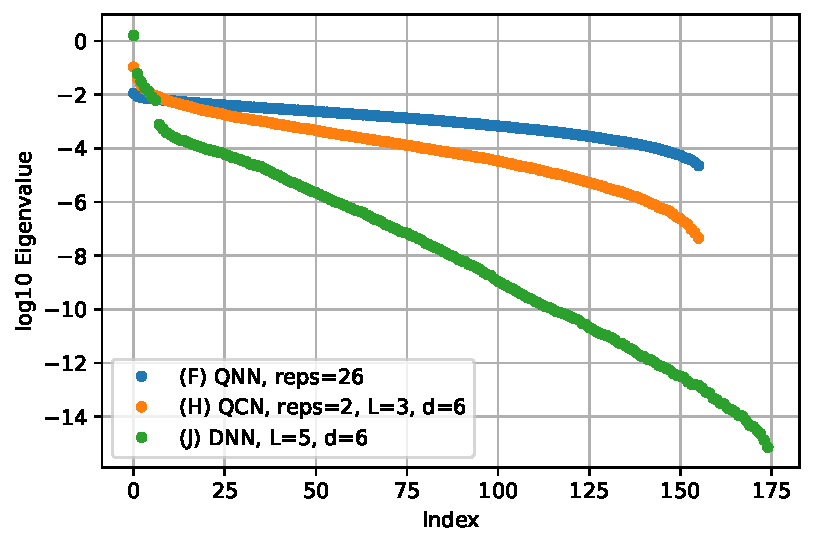
\includegraphics[height=1.9in]{latex/figures/FIM_qubits_6.pdf}
        \caption{Lorem ipsum}
    \end{subfigure}
    \caption{Caption place holder}
    \label{fig:FIM Comparison}
\end{figure}

Returning to \autoref{fig:FIM Comparison}, we see that the spectra of the three layer QCNs exhibit much the same uniformity as the QNNs. A more thorough comparison between different QCNs can be seen in \autoref{fig:FIM QCN}. In this figure, we vary the number of layers of the QNCs and the number of repetitions (i.e. the number of times the ansatz is repeated for each node), while keeping the total number of parameters roughly constant. In doing this, we get to precisely shift how much of the complexity of a given QCN results from the complexity of each node or overall structure of the network. \autoref{fig:FIM QCN a} shows that, for 4 qubit circuits, the spectra of the QNN and different QCNs exhibit roughly the same uniformity. Going up to 6 qubits,  \autoref{fig:FIM QCN b} shows that the spectrum tends to concentrate more around zero the more layers the QCN have. This is likely related to the vanishing of the gradient induced by back propagation. For 4 qubits, this is not as big of a problem since the local gradients are relatively big. However, for 6 qubits, the local gradients are smaller. This results in the gradient vanishing faster when increasing the number of layers, which in turn results in a flatter landscape. At any rate, even for the 5 layer QCN, the landscape is not as badly distorted as for the 5 layer DNN. Further, the few layered QCNs, in particular(ost). 


\begin{figure}[H]
    \centering
    \begin{subfigure}[t]{0.5\textwidth}
        \centering
        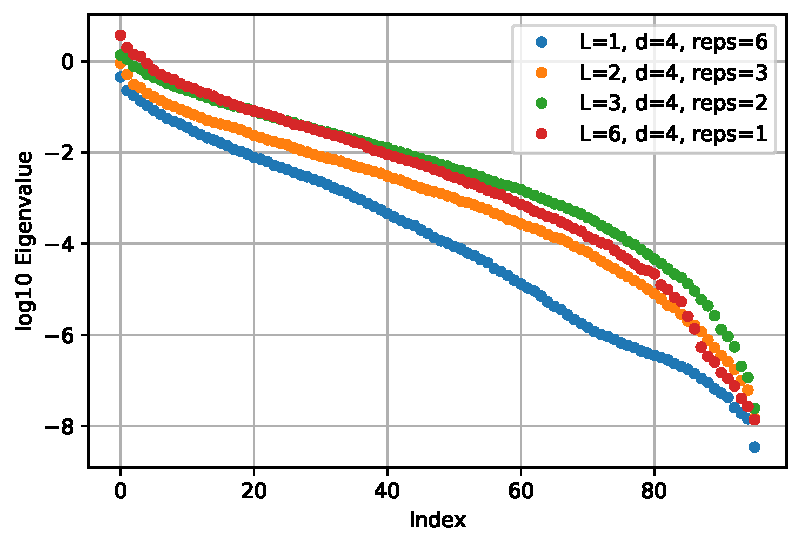
\includegraphics[height=1.9in]{latex/figures/FIM_qubits_4_comparison.pdf}
        \caption{Lorem ipsum}
        \label{fig:FIM QCN a}
    \end{subfigure}%
    ~ 
    \begin{subfigure}[t]{0.5\textwidth}
        \centering
        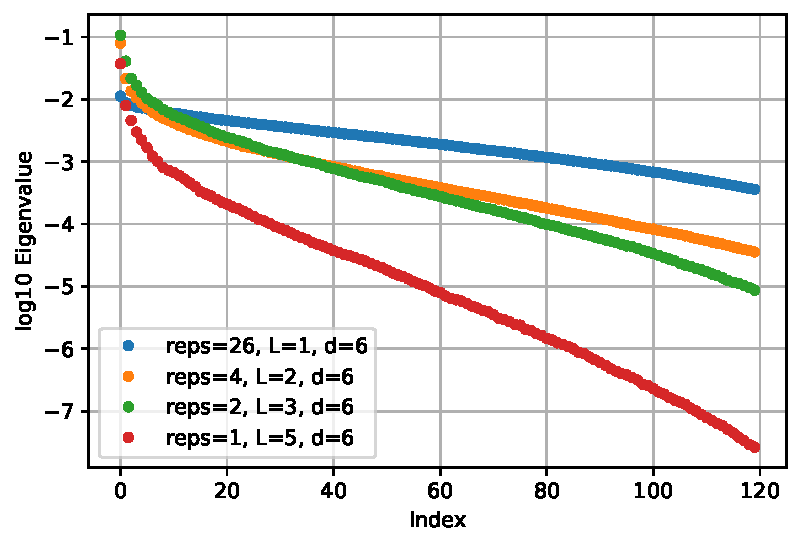
\includegraphics[height=1.9in]{latex/figures/FIM_qubits_6_comparison.pdf}
        \caption{Lorem ipsum}
        \label{fig:FIM QCN b}
    \end{subfigure}
    \caption{Caption place holder}
    \label{fig:FIM QCN}
\end{figure}


%================================================================
\section{Expressivity of Untrained and Trained Models}\label{sec:Expressivity of Untrained and Trained Models}
%================================================================


%================================================================
\section{Training Models on Gaussian Data}\label{sec:Training Models on Gaussian Data}
%================================================================

